\documentclass[acmsmall]{acmart}

\usepackage{caption}
\usepackage{subcaption}
\usepackage{cleveref}

\captionsetup[subfigure]{subrefformat=simple,labelformat=simple}
\renewcommand\thesubfigure{(\alph{subfigure})}


\begin{document}
\title{Denoising Shadows Using Image-to-Image Translation Networks}

\author{Daniel Gerzhoy}
\author{Justin Shen}
\maketitle

\section{Introduction}
\label{sec:intro}

This work reports the work done and results achieved for the final project in CMSC740: Advanced Computer Graphics. We were tasked with using image-to-image translation deep learning networks to add rendering effects, specifically creating low-noise shadows from images rendered with noisy shadows from area lights.

\section{Background}
\label{sec:background}

\subsection{Area Lights and Shadows}

\begin{figure}
	\Description[<short description>]{<long description>}
	\centering
	\subcaptionbox{1 Sample per pixel\label{sf:lowRes}}%
		[0.25\textwidth]{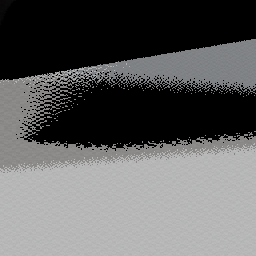
\includegraphics[width=.25\textwidth]{images/lowresshadow.png}}
	\hspace{.05\textwidth}
	\subcaptionbox{16 Samples per pixel\label{sf:hiRes}}%
		[0.25\textwidth]{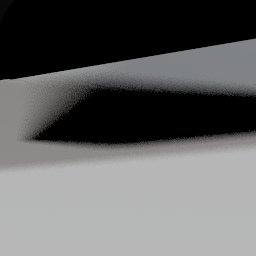
\includegraphics[width=.25\textwidth]{images/highresshadow.png}}
	\caption{Scene rendered with very few samples per pixel vs same scene rendered with more samples. The scene has two lights creating 2 distinct and overlapping shadows. Notice the edges of the shadows are very noisy in the first case}	
	\label{f:ShadowNoise}
\end{figure}

The source of the noisy shadows we seek to denoise is Monte-Carlo rendering. When a ray is drawn from the camera origin and it hits an object in scene, a light is sampled, and a shadow ray is drawn between the hit point and a sampled point on the light. If that ray hits anything in the scene the radiance from the light source does not reach the camera, creating a shadow. For one sample, one hit point is found and one light is sampled X times. If X is low and the light is large, or if the global sample rate is low a hit point might erroneously be cast in shadow because the randomly sampled light point it found was occluded, even if there are points on the lights in view of this hit point. This happens most often closer to the smooth edges of the shadows. Figure \ref{f:ShadowNoise} shows a scene with 2 lights and an object casting 2 overlapping shadows. In fig \ref{sf:lowRes} near the edges of the shadows, there are not enough shadow rays to create smooth shadows, the gradient is very noisy.

\subsection{Original Network}

Description of baseline GANs used for the project.

\section{Data Generation}
\label{sec:datagen}

\subsection{Initial Scenes}
\label{subsec:initScenes}

We began collecting scenes to generate data by looking at the pbrt-v3-scenes repository~\cite{scenes}. We chose a few simple scenes containing area lights to begin with, to extract multiple data points from one scene quickly and automatically, we created a script that would rotate (rotate.py) the lights in the scene around an axis. The intuition for this was that with lights coming at the object from different positions, the network would learn different shadows can come from the same shape.

\subsection{Scene Generator}
\label{subsec:sceneGen}

However it became clear that using real scenes to generate data would take too much time even with automatic light rotation, due to the custom nature of each of the scenes. We then began to experiment with automatically generated scenes by a script (sceneGenerator.py). The basic idea was to create a scene with a floor and insert randomly generated shapes (spheres or cubes) above that floor in random locations, and randomly generated area lights (spherical) above the shapes.

With the location of the floor fixed, the shapes were placed in placed on a 3D grid above the floor (the shape slab) with no shapes occupying the same place. The size of each shape is randomly chosen from a set of sizes chosen so that no shapes overlap, or overlap only a little such that a shape cannot contain the entirety of another shape. Above the plane of the shapes, the area lights are placed similarly on a 3D grid (the light slab). The grid places the shapes and lights at different angles to each other and the floor, creating different shadows each time, in different locations relative to the shapes, and possibly overlapping.

The number of shapes and lights desired is provided as an input to the script, as well as the number of arrangements of shapes and of lights. A significant feature of the scene generator is that every configuration of shapes in the shape slab, is combined with all different configuration of the lights in the light slab. The hope is that seeing the same shape configuration with different shadows, again teaches the network that different shadows come from different shapes.

As we trained and tested the network with the generated scenes (to be discussed in more detail in Section\ref{sec:train} ) we discovered that it was not preserving the original colors and textures of the test scene, so we added random colors and textures to the shapes and floor, hoping that this would teach the network that differently colored and textured shapes create the shadows. We created complex textures by mixing random textures hierarchically. At the bottom level a texture was solid, checkerboard, or polka dots. Those are combined with scaling (multiplication of pixel values for 2 textures), linear interpolation between two textures, checkers, or polka dots.

Finally the scenes could be rotated so that rather than light coming from above and shining down onto a floor, shadows could be cast from area lights behind the camera onto a wall. 

\begin{figure}
	\Description[<short description>]{<long description>}
	\centering
	\subcaptionbox{A vertical view image with complex textures and shapes\label{sf:vert}}%
		[0.25\textwidth]{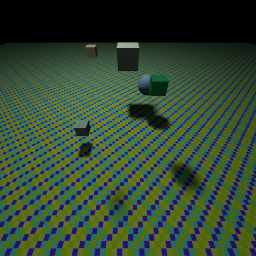
\includegraphics[width=.25\textwidth]{images/gen1.png}}
	\hspace{.05\textwidth}
	\subcaptionbox{A horizontal view image with complex textures and shapes\label{sf:horiz}}%
		[0.25\textwidth]{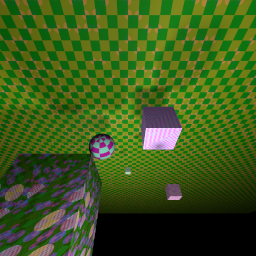
\includegraphics[width=.25\textwidth]{images/gen2.png}}
	\hspace{.05\textwidth}
	\subcaptionbox{Depth Map for vertical view\label{sf:depth}}%
		[0.25\textwidth]{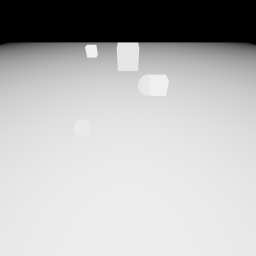
\includegraphics[width=.25\textwidth]{images/gen1_depth.png}}
	\caption{Generated Scenes}	
	\label{f:exampleScenes}
\end{figure}

Figure \ref{sf:vert} and \ref{sf:horiz} show examples of automatically generated scenes with complex textures.

\subsection{Depth Map Generation}
\label{subsec:depthMap}

Creating the depth map was a simple alteration to PBRT. We added a new integrator that before rendering begins calculates from the camera what the maximum distance to any point in the scene is. This is acheived not by checking every vertex in the scene, but by using the points of the bounding volume. The maximum distance is the distance to the furthest point of the bounding volume. Then during renduring -- given a ray, the integrator finds where it intersects the scene and how far along the ray it does so. It then outputs a gray scale value equal to the distance found divided by the max distance. The depth map for \ref{sf:vert} is shown in \ref{sf:depth}. Note that if the depth is found to be infinite (the ray does not intersect the scene) black radiance is returned.

\section{Training}
\label{sec:train}

Training Section

\section{Results}
\label{sec:results}

Results Section

\section{Future Work}
\label{sec:future}

Future Work Section

\section{Conclusion}
\label{sec:conclusion}

\bibliographystyle{unsrt}
\bibliography{mybib}

\end{document}